\chapter{Algorithmentests}\label{chp:AlgoTest}

Dieses Kapitel versucht, Aussagen über die im vorherigen Kapitel beschriebenen 
Algorithmen zu treffen. Dabei geht es primär um die Laufzeit. Um eventuell Aussagen über 
mögliche Vor- und Nachteile oder besonderes Verhalten treffen zu können, wurden auch 
weitere Daten gesammelt. 

\section{Testverfahren}
Zum Testen der Algorithmen wird eine Reihe zufällig erzeugter Graphen verwendet. Um die 
Qualität der Lösungen vergleichen zu können, verwenden alle Algorithmen dieselben Graphen. 
%Für jeden Algorithmus gibt es eine separate Testreihe.

\subsection{Graph-Eigenschaften}\label{GraphEigenschaften}
Sämtliche Graphen sind zusammenhängend und ungerichtet. Weder Knoten noch Kanten 
besitzen eine Färbung, Gewichtung oder Beschriftung. 

Die Graphen unterscheiden sich in zwei Eigenschaften voneinander. Dies sind die Anzahl 
der Knoten $n$ und die durchschnittliche Zahl an Nachbarn eines Knotens $d$. 

\subsection{Durchführung}
Für $n=5$ bis $n=20$ sowie $d=3$ und $d=4$ wird je ein Graph erzeugt. Für 
diese Graphen werden nun paarweise die ECGMs mit minimalen Kosten ermittelt. 
Dabei haben Paare mit einer geringeren Anzahl an möglichen ECGMs (also die 
Anzahl der Permutationen; siehe Abschnitt \ref{Vorueberlegungen}) Vorrang. Dies erlaubt es, Testreihen als Ganzes 
abzubrechen, wenn einzelne Tests bereits abgebrochen werden mussten. Die 
Anzahl $p$ der Permutationen für zwei Graphen mit den Größen $n$ und $m$ 
($n \geq m$) berechnet sich wie folgt: 
\[ p=\frac{n!}{(n-m)!} \]

In Abbildung \ref{pic:PermSize} wird die Anzahl der Permutationen für alle Paare 
dargestellt. Jeder Punkt entspricht dabei einem Graphenpaar. Die X-Koordinate 
ergibt sich aus der Sortierung der Paare nach der Zahl iher Permutationen. Paare 
mit einer kleineren Zahl von Permutationen sind links von Paaren mit größerer Anzahl 
eingezeichnet.
Da die Anzahl exponentiell wächst, wurde eine logarithmische Darstellung der Y-Achse 
gewählt. Sie beginnt bei $10^2$. Die größten Paare besitzen zwischen $10^{18}$ und 
$10^{19}$ mögliche Permutationen und somit mögliche ECGMs. 

\begin{figure}[htb]
\centering
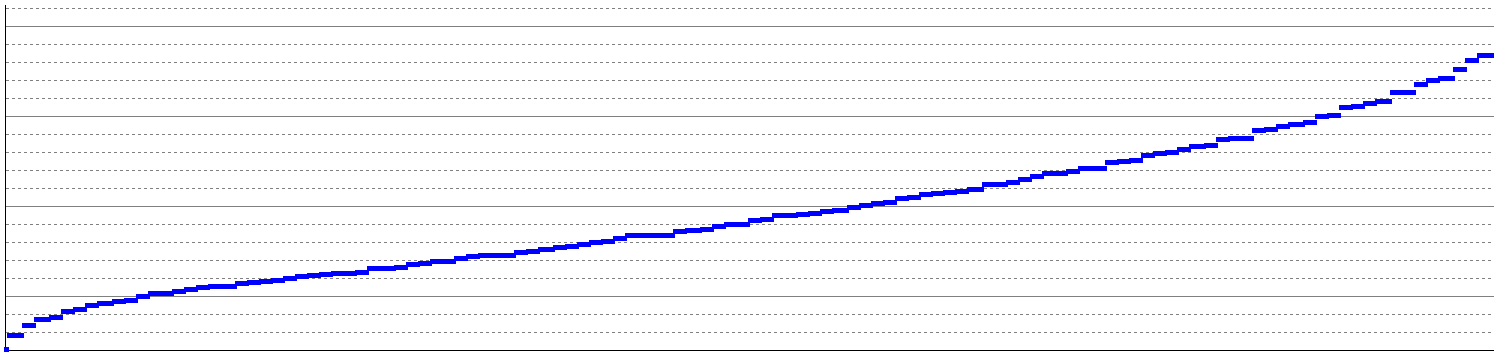
\includegraphics[width=\linewidth,height=\textheight,
keepaspectratio]{bilder/PermSize}
\caption{Anzahl der Permutationen jedes Graphenpaars}
\label{pic:PermSize}
\end{figure}

Die Tests wurden wie oben beschrieben für jeden Algorithmus ausgeführt. Das Testsystem 
war ein 2,4 GHz Doppelkernprozessor mit 4 GB RAM und Windows 7\footnote{Intel(R) Core(TM)2 
Duo T8300 @ 2,40GHz; 4,00 GB RAM; Windows 7 Service~Pack~1 (64 Bit); Windows 
Leistungsindex: Prozessor: 6,0 - RAM: 5,9; Laufzeitumgebung: .NET Framework 2.0}. 

Dauerte ein Test länger als eine Stunde, so wurde er abgebrochen. Wurden zwei Tests 
hintereinander deswegen abgebrochen, so führte dies zum Abbruch der gesamten Testreihe. 
Aufgrund der steigenden Zahl der Permutationen ist nicht zu erwarten, dass spätere Tests 
erfolgreicher sind. 

\subsection{Darstellung der Ergebnisse}
Um den Platz besser zu nutzen, wurde bei der Darstellung der Testergebnisse auf eine 
Achsenbeschriftung verzichtet. Aus diesem Grund folgt eine kurze Beschreibung der 
Darstellungen. Abbildung \ref{pic:cordExplain} stellt dies zusätzlich graphisch dar. 

\begin{figure}[htb]
\centering
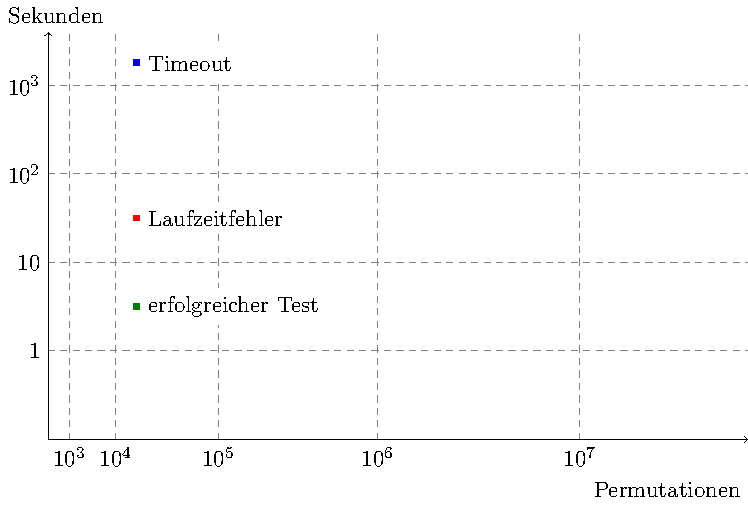
\includegraphics[width=\linewidth,height=\textheight,keepaspectratio]{bilder/empty.pdf}
%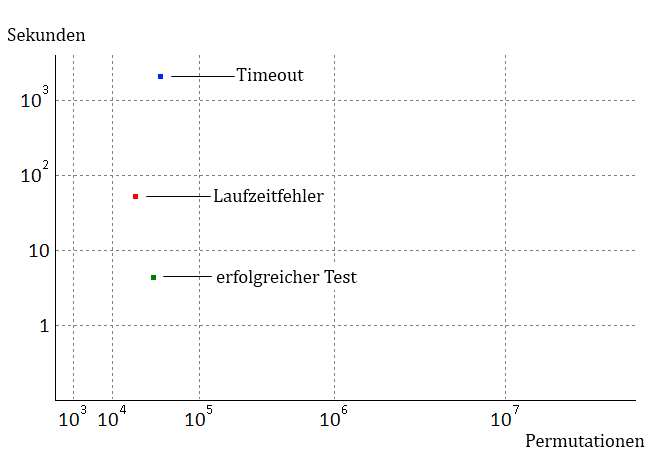
\includegraphics{bilder/empty}
\caption{Das verwendete Koordinatensystem}
\label{pic:cordExplain}
\end{figure}

\subsubsection{X-Achse}
Die Position auf der X-Achse ergibt sich aus der Position eines Tests in der 
dazugehörigen Testreihe. Da die Tests nach Anzahl ihrer Permutationen sortiert 
wurden (dargestellt in Abbildung \ref{pic:PermSize}), gibt die X-Achse diese auch 
indirekt an. Die senkrechten Hilfslinien verdeutlichen dies. Eine Hilfslinie wurde 
immer dann eingefügt, wenn die Anzahl der Permutationen eine ganzzahlige Zehnerpotenz 
überschritten hat. 

\subsubsection{Y-Achse}
Die Y-Achse stellt die Zeit in Sekunden dar, die ein Test benötigt hat. Die Einteilung 
ist logarithmisch. Begonnen wird bei $0{,}1$ Sekunden. Liegt die gemessene Laufzeit niedriger oder 
wurden gar $0{,}0$ Sekunden gemessen, so wird die Laufzeit als $0{,}1$ Sekunden behandelt. 

Die waagerechten Hilfslinien stellen die jeweils nächste Zehnerpotenz dar. So ist die 
erste Hilfslinie über der X-Achse bei $1$~Sekunde, die Zweite bei $10$~Sekunden, usw. 

\subsubsection{Farbgebung}
Jeder durchgeführte Test wird durch einen Punkt im Koordinatensystem dargestellt. Tests 
können jedoch zu unterschiedlichen Ergebnissen führen. Die Farben der Punkte stellen dies 
dar. Ist ein Test erfolgreich, wird er in \emph{grün} dargestellt. Ein \emph{blauer} 
Punkt bedeutet, dass der Test abgebrochen wurde, weil er die maximale Laufzeit 
überschritten hat. Ist der Punkt \emph{rot}, dann ist beim Test ein Fehler aufgetreten. 


\section{Testergebnisse}

\subsection{McGregor und MIS basierter Algorithmus}

\begin{figure}[htb]
\centering
\hspace*{\fill} %
\subfloat[McGregor-Alg. \label{pic:McGregor}]{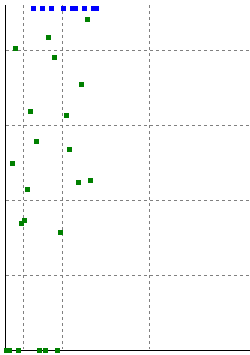
\includegraphics[width=0.25\linewidth,
keepaspectratio]{bilder/McGregor_part}}
\hspace*{\fill} %
\subfloat[MIS basierter Alg. \label{pic:MaxIndSet}]{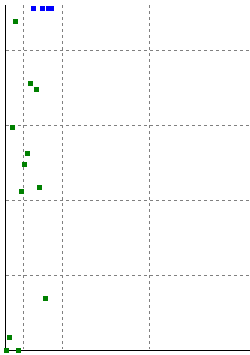
\includegraphics[width=0.25\linewidth,
keepaspectratio]{bilder/MaxIndSet_part}}
\hspace*{\fill} %
\caption{Test des McGregor- und des MIS basierten Algorithmus}
\label{pic:MG_MIS}
\end{figure}

Für beide hier dargestellten Algorithmen zeigt sich, dass sie selbst bei kleinen 
Graphen eine hohe Laufzeit haben. Die Testreihe wurde somit auch schon sehr früh 
abgebrochen. 

Die Streuung lässt sich durch zwei Eigenheiten erklären. 
Zum einen sind beide 
Algorithmen in einigen Fällen in der Lage eine optimale Lösung zu erkennen. Dann wird 
die Suche vorzeitig abgebrochen. 

Zum anderen 
arbeiten beide Algorithmen mit Kantengraphen. Dadurch, dass Kanten als Knoten behandelt 
werden und ein induzierter Teilgraph gesucht wird, ist die Anzahl der zu testenden 
Abbildungen eine andere als bei der Suche nach ECGMs auf "`normalen"' Graphen. Somit 
ist es möglich, dass Graphenpaare mit mehr Abbildungen vor Paaren mit weniger 
getestet werden.

\subsection{Probieren aller Permutationen}
\begin{figure}[htb]
\centering
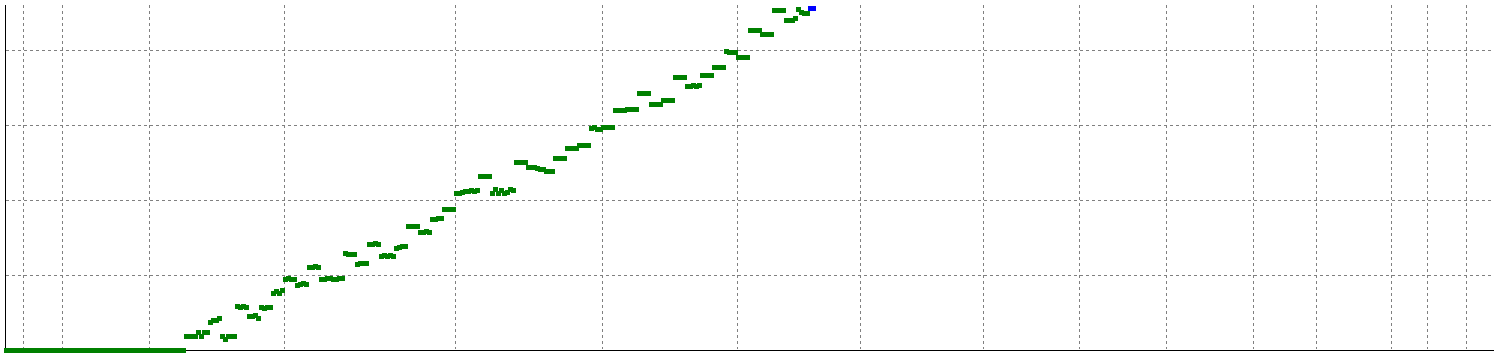
\includegraphics[width=\linewidth,height=\textheight,
keepaspectratio]{bilder/Permut}
\caption{Probieren aller möglichen ECGMs}
\label{pic:Permut}
\end{figure}

Der Zeitaufwand für das Durchprobieren aller Permutationen ist direkt von deren Anzahl 
abhängig. Da beide Achsen (annähernd\footnote{Die X-Achse ist nur nährungsweise logarithmisch 
eingeteilt. Dies liegt daran, dass die Anzahl der Permutationen der Graphenpaare nicht 
gleichmäßig steigt. Bei gleichmäßigem Anstieg würde Abbildung \ref{pic:PermSize} eine Gerade 
darstellen. Die Krümmung ist jedoch nur gering, weshalb die Steigerung nährungsweise als 
gleichmäßig angesehen werden kann.}) logarithmisch unterteilt sind, bilden die 
Laufzeiten der Tests annährend eine Gerade.

Die leichte Streuung liegt vermutlich an 
der iterativen Berechnung der nächsten Permutation anhand der aktuellen. Sind zwei 
Graphen unterschiedlich groß, so gibt es Permutationen, die das gleiche ECGM darstellen. 
Somit muss beim Erzeugen der nächsten Permutation darauf geachtet werden, dass die 
nächste Permutation auch ein neues ECGM ergibt. Dies erfordert etwas zusätzliche Rechenleistung. 
Ein rekursives Verfahren, welches die ECGMs mittels Backtracking ermittelt und nicht als 
Permutation betrachtet, könnte dazu führen, dass die Streuung geringer ist. 

Bis zu einer Größe von etwa $1{,}8 \cdot 10^6$ Permutationen ($n=10$; $m=8$) liegt die 
Laufzeit bei rund einer Sekunde. Fünf Sekunden werden mit $6{,}7 \cdot 10^6$ Permutationen 
($n=11$; $m=8$) nicht überschritten. Bei Graphenpaaren dieser Größe ist es also durchaus 
möglich, dieses Verfahren einzusetzen ohne die Geduld des Nutzers zu sehr zu belasten. 

\subsection{Branch-and-Bound (und A*)}\label{BBTest}
Das B\&B-Verfahren konnte die Testreihe vollständig durchlaufen. Kein Test musste 
abgebrochen werden, weil er über eine Stunde dauerte. Jedoch wurden viele Tests 
abgebrochen, weil die Laufzeitumgebung einen Fehler meldete (rote Punkte). Die Ursache 
dafür war das Verbrauchen von zu viel Speicher. 

\begin{figure}[htb]
\centering
\noindent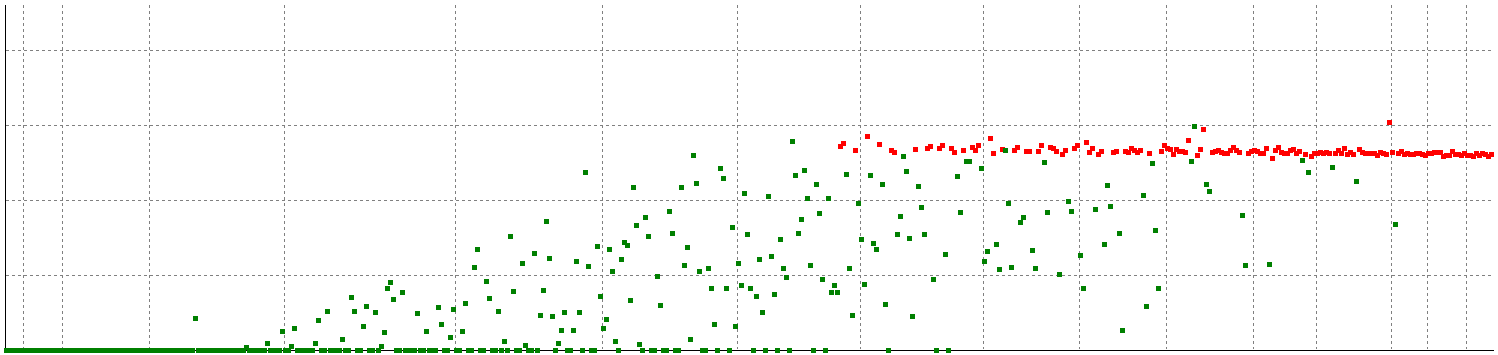
\includegraphics[width=\linewidth,height=\textheight,
keepaspectratio]{bilder/B&B}
\caption{Test des Branch-and-Bound-Verfahrens}
\label{pic:B&B}
\end{figure}

Auf den ersten Blick fällt die starke Streuung der Ergebnisse auf. Das Verfahren kann 
sehr schnell zu einem Ergebnis führen. So wurde für ein Graphenpaar mit etwa $1{,}8 \cdot 
10^{14}$ Permutationen ($n=17$; $m=15$) in $1{,}4$~Sekunden verglichen. Das erste Graphenpaar 
mit mehr als fünf Sekunden Laufzeit besitzt hingegen nur etwa $3{,}9\cdot 10^7$ 
Permutationen ($n=11$; $m=10$). Es benötigte $8{,}0$ Sekunden. 

Ebenfalls auffällig ist, dass es keine Gruppenbildung gibt. Zu jeder Anzahl an Knoten 
$n$ gibt es zwei Graphen mit unterschiedlicher Anzahl an Kanten ($d=3$ und $d=4$). 
Bei der Berechnung 
der möglichen Permutationen wird nur die Anzahl der Knoten herangezogen. Somit bilden 
sich in einer Testreihe Gruppen von jeweils zwei bzw. vier Graphenpaaren, welche die gleiche  
Anzahl an Permutationen besitzen (gut zu sehen in Abbbildung~\ref{pic:Permut}). Innerhalb 
einer solchen Gruppe unterscheiden sich die Paare nur durch die Anzahl der Kanten.
Da die Anzahl der Kanten allerdings bei der Berechnung der Schranke des B\&B-Verfahrens 
eine Rolle  spielt, liegt es somit nahe, dass die Anzahl der Kanten einen Einfluss auf 
die Rechenzeit hat.

Abbildung~\ref{pic:BBcomp} stellt erneut die Laufzeit des B\&B-Verfahrens in einem 
Ausschnitt\footnote{Die X-Achse geht von $10^6$ bis $10^{14}$ Permutationen, die 
Y-Achse von $0{,}1$ bis $100$ Sekunden.} dar. Die Färbung ist aber eine andere. Tests, 
bei denen der kleinere Graph eine geringe Kantendichte hat ($d=3$, siehe 
Abschnitt~\ref{GraphEigenschaften}) sind \emph{blau} dargestellt. Tests mit einer größeren 
Kantendichte ($d=4$) sind \emph{rot}. Wegen zu hohem Speicherverbrauch abgebrochene 
Tests wurden nicht eingezeichnet.

\begin{figure}[htb]
\centering
\noindent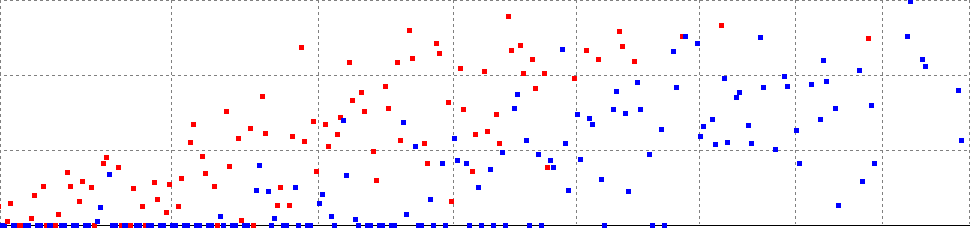
\includegraphics[width=\linewidth,height=\textheight,
keepaspectratio]{bilder/BBcomp}
\caption{B\&B-Laufzeit abhängig von der Kantendichte des kleineren Graphen}
\label{pic:BBcomp}
\end{figure}

Es ist deutlich zu sehen, dass blau markierte Tests in der Regel schneller sind als 
die roten. Beide Bereiche überlappen sich jedoch. Auch die Streuung ist bei beiden 
Varianten vorhanden. 

Dass die Kanten einen Einfluss auf die Schranke und somit auf die Laufzeit haben, 
führt zu einer weiteren Vermutung. Eventuell lässt sich die Laufzeit verringern, indem 
der Suchbaum die Knoten in Abhängigkeit ihrer anliegenden Kanten (also der Zahl ihrer 
Nachbarn) zuweist. Um dies zu überprüfen, wurde der Algorithmus leicht geändert. Vor 
der eigentlichen Suche werden die Knoten nach der Anzahl ihrer Nachbarn sortiert. Es gab zwei 
Testreihen. Eine begann den Suchbaum mit Knoten, die möglichst wenig Nachbarn hatten. 
Die Andere mit möglichst vielen. Dabei brachte die Testreihe, die Knoten mit vielen 
Nachbarn zuerst zuwies, den gewünschten Effekt. Abbildung \ref{pic:BB_Nh} stellt das 
Ergebnis dar. Das vorrangige Zuweisen der Knoten mit wenig Nachbarn führte hingegen 
zu einer Erhöhung der Laufzeit. 

\begin{figure}[htb]
\centering
\noindent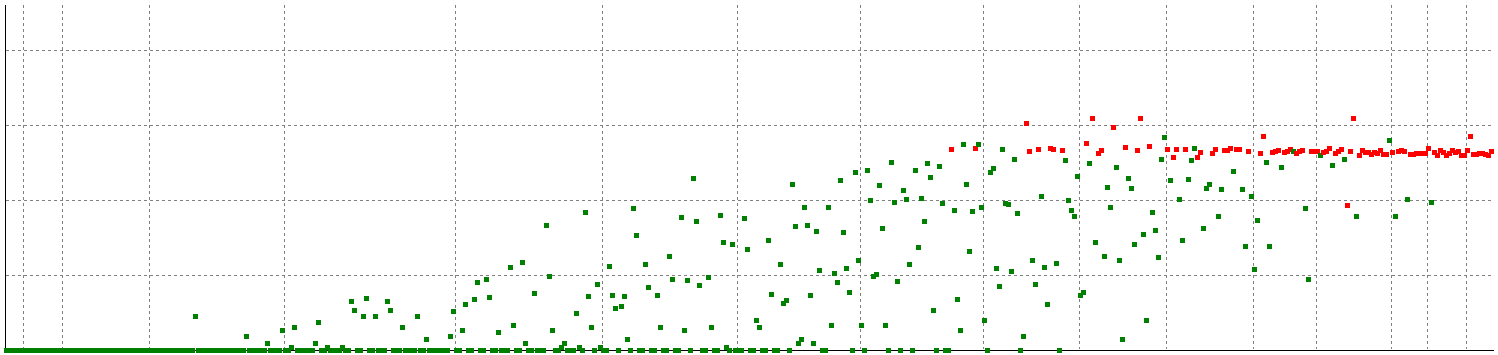
\includegraphics[width=\linewidth,height=\textheight,
keepaspectratio]{bilder/BB_Nh}
\caption{B\&B-Laufzeit, wenn Knoten mit vielen Nachbarn zuerst zugewiesen werden}
\label{pic:BB_Nh}
\end{figure}

Da die Streuung weiterhin vorhanden ist, lässt sich aus Abbildung \ref{pic:BB_Nh} nur 
schlecht sagen, ob die Verbesserung mehrheitlich ist oder nur bestimmte Graphenpaare 
betrifft. Abbildung \ref{pic:BBdif} stellt deswegen die Differenz der Laufzeiten dar. 
\emph{Rote} Punkte entsprechen dabei einer Verschlechterung der Laufzeit. Dies kann auch 
bedeuten, dass ein Test abgebrochen wurde, der vorher erfolgreich war. Hat sich die 
Laufzeit verbessert bzw. war ein Test erfolgreich, der zuvor abgebrochen werden musste, 
so wird der Punkt \emph{grün} dargestellt. 
Musste für ein Graphenpaar in beiden Testreihen der Test abgebrochen werden oder liegt 
die Zeitdifferenz unter $0{,}1$ Sekunden, ist der Test nicht eingetragen. 

\begin{figure}[htb]
\centering
\noindent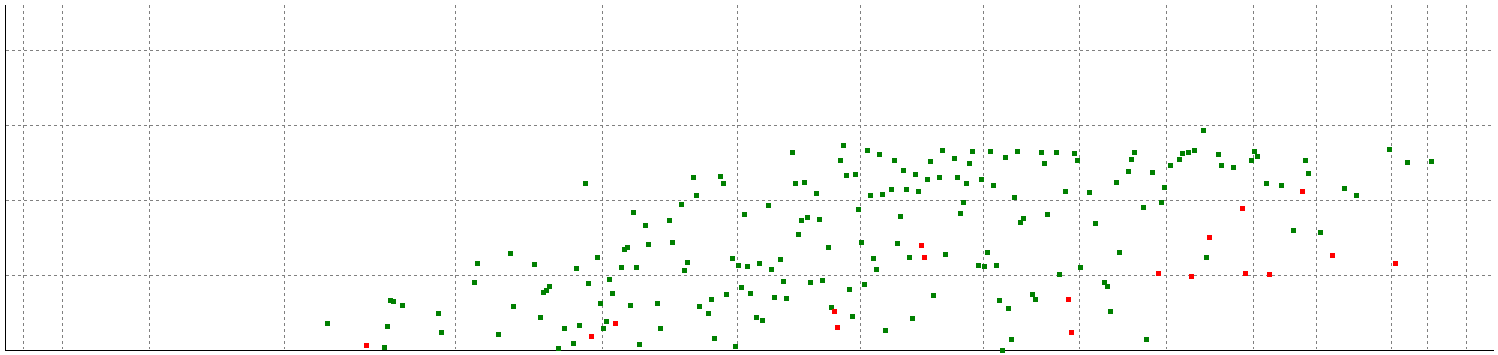
\includegraphics[width=\linewidth,height=\textheight,
keepaspectratio]{bilder/BBdif}
\caption{Laufzeitdifferenz der B\&B-Testreihen}
\label{pic:BBdif}
\end{figure}

Man kann klar erkennen, dass die überwiegende Mehrheit der Tests besser verlief. Es 
gibt aber auch Tests, die schlechter abschnitten. Es kann also nicht von einer 
generellen Verbesserung gesprochen werden. 

Das Fazit für das B\&B-Verfahren fällt weitgehend gut aus. Es ist ein exaktes Verfahren, 
welches für Graphenpaare mit niedriger und mittlerer Zahl an Permutationen in der 
Regel schnell zu einem Ergebnis führt. Das Vorsortieren der Knoten nach der Anzahl 
ihrer Nachbarn erhöht dabei die Wahrscheinlichkeit für eine kurze Laufzeit. Nachteilig 
an B\&B ist, dass es eine sehr starke Streuung besitzt. Es ist somit nur schwer 
vorhersagbar, wie lange die Berechnung für ein konkretes Graphenpaar dauert. 

\subsection{Evolutionärer Algorithmus}

Beim Testen des evolutionären Algorithmus wurde eine Population vom $1.000$ Individuen 
verwendet. Bei Mutation und Rekombination werden jeweils $1.000$ weitere Individuen 
erzeugt. Die Selektion wählt aus den nun $3.000$ Individuen die $1.000$ Besten aus. Die 
Anderen "`sterben"'. Ein Individuum wird als Optimum betrachtet, wenn nach 20 
Generationen kein besseres gefunden wurde. 

\subsubsection{Laufzeit}

\begin{figure}[htb]
\centering
\noindent\includegraphics[width=\linewidth,height=\textheight,
keepaspectratio]{bilder/evo}
\caption{Laufzeiten des evolutionären Algorithmus}
\label{pic:evo}
\end{figure}

Mittelst des evolutionären Algorithmus konnte zu jedem Paar eine 
mögliche Lösung ermittelt werden. Die Laufzeit bleibt auch bei einer hohen Anzahl 
an Permutationen verhältnismäßig gering. Das erste Graphenpaar, welches über fünf 
Sekunden benötigt, besitzt etwa $1{,}3 \cdot 10^{15}$ Permutationen ($n=15$; $m=14$). 
Die höchste Laufzeit betrug $18{,}4$ Sekunden. Das dazugehörige Graphenpaar hat etwa 
$2{,}4 \cdot 10^{18}$ mögliche Permutationen ($n=20$; $m=19$). 
 
Die sichtbare Streuung könnte zwei mögliche Ursachen haben. Zum einen ist es denkbar, 
dass die unterschiedliche Kantendichte sich auf die Zeit auswirkt. Zum anderen 
werden die Paare für eine Rekombination sowie die Änderung bei einer Mutation zufällig 
bestimmt. Ob und wann eine bessere Lösung gefunden wird, ist somit auch vom Zufall 
abhängig. 

\subsubsection{Qualität der Lösung}
Da es sich bei einem evolutionären Algorithmus nicht um ein exaktes Verfahren handelt, 
ist es nötig, die Qualität der Lösung zu betrachten. Maßgabe für die Qualität ist das  
Verhältnis der Anzahl gefundenen gemeinsamen Paare mit Kante in der exakten Lösung zur Anzahl 
in der Lösung des evolutionären Algorithmus. 

Abbildung \ref{pic:EvoQuali} stellt das Verhältnis zwischen beiden Lösungen dar. Es wurde erneut  
auf die Beschriftung verzichtet. Das Koordinatensystem unterscheidet sich jedoch von bisherigen 
Darstellungen. Die Y-Achse stellt nun das Verhältnis zwischen exakter und evolutionär ermittelter 
Lösung dar. Die Achse ist nicht mehr logarithmisch. Im Koordinatenursprung sind es $0\%$. 
Waagerechte Hilfslinien sind jeweils in $10\%$-Schritten eingezeichnet. Die X-Achse sowie die 
senkrechten Hilfslinien wurden nicht verändert. Die Farbgebung gibt zusätzlich Auskunft über die 
Zahl der gemeinsamen Paare ohne Kante. Stimmt sowohl die Zahl der Paare mit Kante als auch die 
Zahl der Paare ohne Kante mit der exakten Lösung überein, ist der Test \emph{grün} dargestellt. 
Andere Tests sind \emph{blau}. 

Da nicht für alle Graphenpaare eine exakte Lösung vorliegt, ist es auch nicht möglich zu 
jeder Lösung des evolutionären Algorithmus eine Qualität anzugeben. Die entsprechenden 
Graphenpaare sind somit nicht in Abbildung \ref{pic:EvoQuali} eingetragen. 

\begin{figure}[htb]
\centering
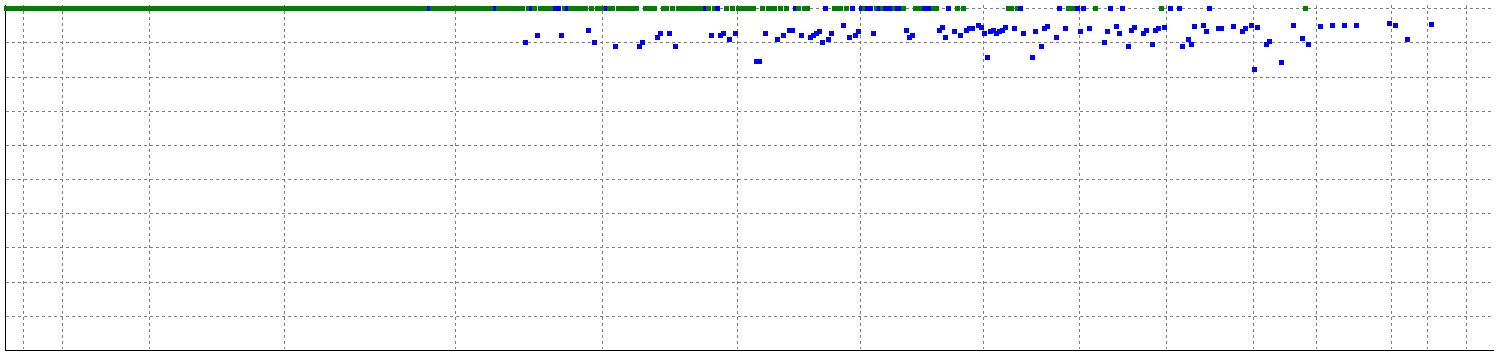
\includegraphics[width=\linewidth,height=\textheight,
keepaspectratio]{bilder/evoQuali}
\caption{Qualität der Lösungen des evolutionären Algorithmus}
\label{pic:EvoQuali}
\end{figure}

Der Evolutionäre Algorithmus liefert durchgehend gute Lösungen. Die erste Lösung unter 
$100\%$ tritt bei einem Graphenpaar mit etwa $2{,}8 \cdot 10^7$ Permutationen ($n=20$; $m=6$) 
auf. Bis etwa $10^{11}$ Permutationen haben jedoch ein Großteil der Lösungen eine 
Qualität von $100\%$. Die Mehrheit der Lösungen, die nicht vollständig übereinstimmen, 
haben eine Qualität über $90\%$. Auch schlechtere Lösungen unterschreiten die $80\%$ 
nicht. Da nicht zu jedem Paar eine Lösung bekannt ist, lässt sich jedoch nicht sagen, 
ob generell die Qualität der Lösungen so gut ist. Es ist denkbar, dass die selben 
Eigenschaften, die dazu führen, dass B\&B keine Lösung liefert, auch eine Lösung 
mit schlechter Qualität beim evolutionärem Algorithmus zur Folge haben.

\subsection{Bipartites Matching}
Die Ermittlung einer Lösung mittels bipartitem Matching ist im Vergleich zu den anderen 
getesteten Verfahren sehr schnell. Zu allen Graphenpaaren wurde in unter $0{,}1$ Sekunden 
eine Lösung ermittelt. Auf eine Darstellung der Laufzeit wird deshalb verzichtet. 

Interessant ist die Qualität der Lösungen, denn es handelt sich um eine Heuristik. Es 
wurde jedoch nicht das Gewicht des Matchings genommen, da es nur eine Schätzung ist und nicht 
die realen Kosten angibt. Stattdessen werden die gemeinsamen Paare genommen, 
die sich durch das Matching ergeben. Abbildung \ref{pic:BipQuali} stellt die Qualität 
des Verfahrens dar. Die Darstellung ist analog zur Qualitätsdarstellung des evolutionären 
Algorithmus. 

\begin{figure}[htb]
\centering
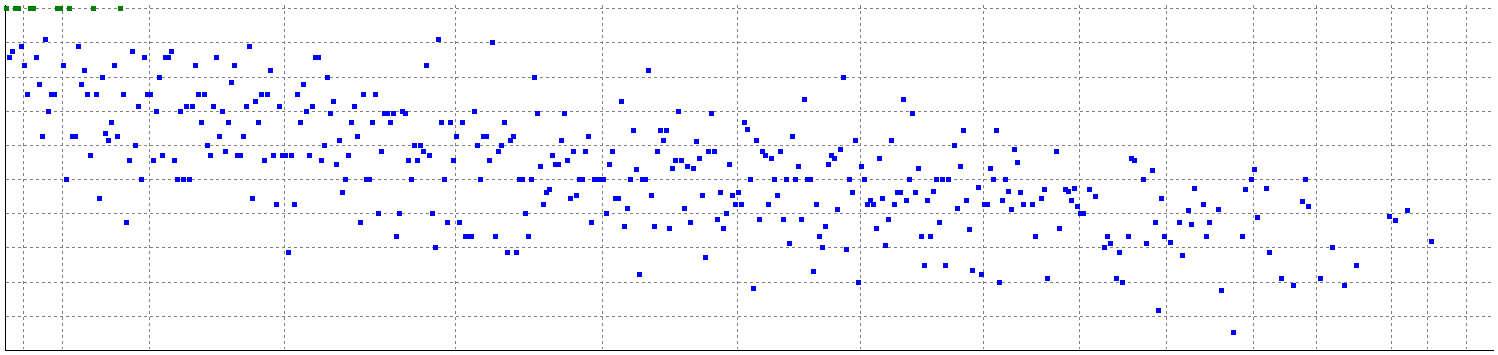
\includegraphics[width=\linewidth,height=\textheight,
keepaspectratio]{bilder/bipQuali}
\caption{Qualität der Lösungen des bipartiten Matchings}
\label{pic:BipQuali}
\end{figure}

Neben der starken Streuung der Ergebnisse sieht man auch, dass die Qualität bei größeren 
Graphenpaaren deutlich abnimmt. Eine mögliche Erklärung für die Abnahme ist, dass die 
Zahl der Kanten in den Graphen linear mit deren Größe steigt. Die Anzahl der Knotenpaare 
steigt jedoch quadratisch. Die Wahrscheinlichkeit, dass bei zwei Knotenpaaren auch beide 
eine Kante besitzen, nimmt somit ab.

Abbildung \ref{pic:RndQuali} stellt die Qualität einer weiteren Testreihe dar. Hierbei 
wurden bei jedem Test zehn zufällige Permutationen erstellt und die Beste dann als Lösung 
ausgegeben. Es ist zu sehen, dass die Qualität der mittels bipartitem Matching ermittelten 
Lösung sich kaum von der Qualität der zufällig erzeugten Lösungen unterscheidet. 

\begin{figure}[htb]
\centering
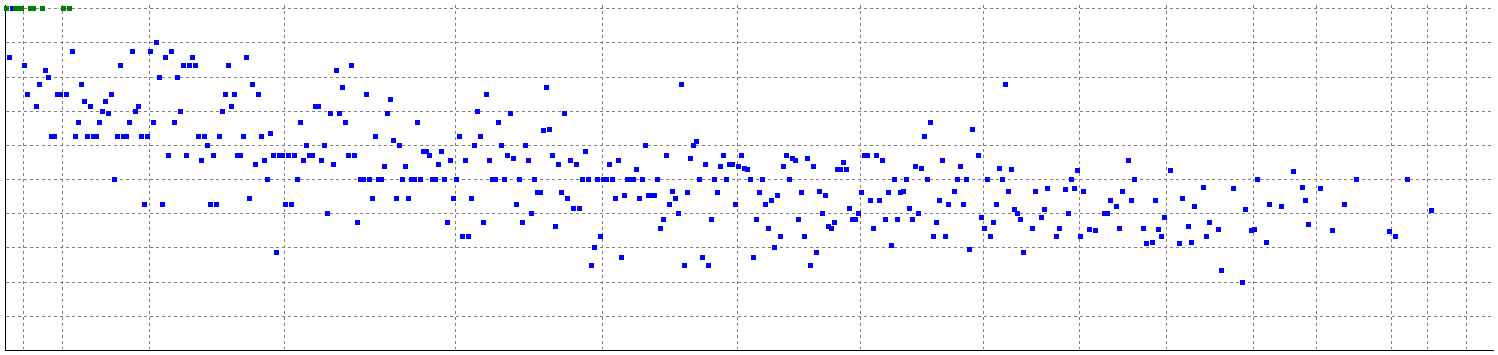
\includegraphics[width=\linewidth,height=\textheight,
keepaspectratio]{bilder/rndQuali}
\caption{Qualität von zufälligen Lösungen}
\label{pic:RndQuali}
\end{figure}

Das Fazit für das bipartite Matching fällt negativ aus. Zwar ist es ein sehr schnelles 
Verfahren, jedoch führt die Heuristik nicht zu Lösungen mit hoher Qualität. Die Qualität 
ist auch nicht besser als zufällig ermittelte Lösungen. 
